\documentclass{article}

\usepackage{rtex}
\usepackage{enumitem}
\usepackage{minted}
\usepackage{fontspec}
\usepackage[letterpaper, portrait, margin=1in]{geometry}
\setmonofont{Jetbrains Mono}

\begin{document}

\rtitle{PHYS 403 Summary}{Reese Critchlow}

\header{Probability Review}

\sheader{Binomial Distributions} Recall that the binomial distribution is:
\begin{align*}
  P_k^N = \frac{1}{2^N} {N\choose{K}} \approx \frac{1}{\sqrt{\pi N}} e^{- \frac{\left(k- \frac{N}{2}\right)^2}{2N}}
\end{align*}
And hence, it is important to note that the width of the gaussian (standard) is $\Delta = \sqrt{N}$.
\sheader{Fluctuations} We speak a lot in statistical mechanics about ``fluctuations'' in a quantity from the mean. These are given by:
\begin{align*}
  \frac{\sqrt{\text{Var}(M)}}{\left| \langle M \rangle \right|}.
\end{align*}
For some quantity $M$. For a binomial distribution, this generally is $\approx \frac{1}{\sqrt{N}}$.
\gap
\header{Entropy}

We can describe entropy for a system as an ``expected amount of surprise''. Hence, entropy is maximized when each state occurs with equal chance. For some system with states $\alpha$ with probability $P_\alpha$, we can calculate the entropy in the following ways:
\begin{align*}
  S &= \sum_{\alpha} P_\alpha \log \left(\frac{1}{P_\alpha}\right)\\
  &= k_B \ln \Omega
\end{align*}
Where $\Omega$ is the multiplicity of microstates for a system.
\gap
This also brings us to the 2nd law of thermodynamics: \textit{Entropy is non-decreasing}.
\gap
\header{Microcanonical Ensemble}
The microcanonical ensemble is a system for which its total energy is exactly specified. No energy or particles can move in or out of the system.
\gap
Putting two systems (1 and 2) in contact, forming a microcanonical ensemble gives us the a method for defining temperature in the \textit{microcanonical ensemble}:
\begin{align*}
  \frac{dS}{dE} = \frac{1}{T}.
\end{align*}
This helps to demonstrate thermal equilibrium, as if one is maximizing entropy of the two systems, we arrive at the following:
\begin{align*}
  \delta S &= \delta S_1 + \delta S_2 \\
  &= -\frac{dS_1}{dE}\delta E + \frac{dS_2}{dE}\delta E\\
  &= \delta S \left(-\frac{dS_1}{dE} + \frac{dS_2}{dE}\right) \delta E
\end{align*}
and hence, since we desire $\delta S = 0$, then:
\begin{align*}
  \frac{dS_1}{dE} = \frac{dS_2}{dE} \implies T_1 = T_2.
\end{align*}
This can also bring us to a definition for specific heat:
\begin{align*}
  C = \frac{dE}{dT}.
\end{align*}
\header{Canonical Ensemble}
The canonical ensemble is a microcanonical ensemble that is allowed to exchange energy.
\gap
In this ensemble, it is useful to determine what the probability of finding this system in a given state is. Let there be two systems (1 and 2) and where system 2 is much larger than system 1. Hence, we can derive the probability of a given energy state $E_i$:
\begin{align*}
  &S_2(E-E_i) = k \ln \Omega\\
  \implies &\Omega_2 = e^{\frac{1}{k}S_2(E-E_i)}\\
  \implies &p_i = \frac{\Omega_2}{\Omega_T} = \text{constant} \cdot e^{\frac{1}{k} S_2(E-E_i)}
\end{align*}
Since $E_i \ll E$, then we can Taylor expand:
\begin{align*}
  S_2(E - E_i) &\approx S_2(E) - E_i \frac{dS_2}{dE}(E)\\
  S_2(E - E_i) &\approx \text{constant} - \frac{E_i}{T}\\
  \implies p_i &= \text{constant} \cdot e^{-\frac{E_i}{kT}}
\end{align*}
If we require that all probabilities sum to zero, we define the \textit{partition function} and thus the probability of a given state:
\begin{align*}
  p_i &= Z^{-1}e^{-\frac{E_i}{kT}} & Z = \sum_{i} e^{-\frac{E_i}{kT}}
\end{align*}

From the partition function, we can also derive some important quantities. Let $\beta = kT$.
\begin{align*}
  \bar{E} &= -\frac{1}{d\beta}\ln(Z) & \text{Var}(E) = \left( - \frac{d}{d\beta}\right)^2 \ln(Z)
\end{align*}
Entropy can also be described in the Helmholtz Free Energy:
\begin{align*}
  -kT \ln Z = \bar{E} - TS.
\end{align*}
\header{Ideal Gases}
If we use the quantum mechanical energy formula for 1D particles in a box and assume non-interacting particles, we define the energy for an individual particle:
\begin{align*}
  E = \frac{\hbar^2\pi^2}{2mL^2}(n_x^2 + n_y^2 + n_z^2)
\end{align*}
and hence, we can create a partition function:
\begin{align*}
  Z = \left(\sum_{n}e^{-\frac{\hbar^2\pi^2\beta}{2mL^2}n^2}\right)^3
\end{align*}
In the limit of low temperatures, the largest energy terms dominate the sum. In the high temperature limit, we can approximate the sum in $Z$ as an integral:
\begin{align*}
  Z &\approx \left( \int_{0}^{\infty} e^{-\frac{\hbar^2\pi^2\beta}{2mL^2}n^2} dn \right)^3\\
  &= \frac{V}{h^3} \left( \frac{2\pi m}{\beta}\right)^{3/2}
\end{align*}
This is where we get that:
\begin{align*}
  \bar{E} &= \frac{3}{2}kT & \text{Var}(E) = \frac{3}{2}k^2T^2
\end{align*}
An important question to answer is that of the probability of velocities for the particles. We can find this in the following way:
\begin{align*}
  p\left( \left[v, v + dv\right]\right) = p_\text{state} \cdot \text{\# of states in } [v, v + dv]
\end{align*}
And such, we know that:
\begin{align*}
  p_\text{state} = \frac{1}{Z}e^{-\beta \cdot \frac{1}{2}mv^2}
\end{align*}
And the number of states is expressed as:
\begin{align*}
  \text{fraction of volume} \cdot \text{differential surface area} \cdot \text{thickness}
\end{align*}
and the thickness is generally:
\begin{align*}
  \text{thickness} = \frac{dv}{d|\vec{n}|}.
\end{align*}
After all of this, we arrive at the Maxwell-Boltzmann distribution of speeds:
\begin{align*}
  p \left( [v, v + dv]\right) = \frac{4}{\sqrt{\pi}} \left(\frac{m}{2kT}\right)^{3/2} \cdot v^2 e^{-\frac{mv^2}{2kT}}dv
\end{align*}
We could have also derived this in a classical mechanics approach, by integrating over the momentum-position space instead of the state space, where the resolution of each point is $1/h^3$.
\gap
These idealizations were fun, but one should also note that the actual partition function usually needs to consider internal states of a particle, and such, a partition function might look like:
\begin{align*}
  Z = Z_\text{motion}^N \cdot Z_{\text{internal}}^N
\end{align*}
\sheader{Gas Pressures} we can say that the pressure is the energy transferred to a gas per unit change in volume:
\begin{align*}
  p = \frac{dW}{dV}
\end{align*}
There also exists the \textit{adiabatic theorem}, which states that \textit{for slow change of parameter of a system in state $i$, the system remains in state $i$}. This implies that the $p_i$s don't change. From this, we can write the second law in another way:
\begin{align*}
  d\bar{E} = \sum_i p_i dE_i + \sum_i E_i dp_i = -W + Q
\end{align*}
This all combines to get:
\begin{align*}
  p = \frac{dW}{dV} = - \left(\frac{dF}{dV}\right)_T
\end{align*}
If we take this derivative from $F = -kT \ln Z$, we get back the ideal gas law:
\begin{align*}
  P = kT \frac{N}{V} \implies PV = nRT
\end{align*}
(recall that $N_Ak = R$). And we can also retrieve the first law:
\begin{align*}
  d\bar{E} = TdS - PdV
\end{align*}
\vfill\pagebreak 
\header{Thermodynamic Relations}
Basically, you have the first law:
\begin{align*}
  dE = TdS - PdV
\end{align*}
From there you have all of the other potentials:
\begin{align*}
  F &= E - TS\\
  H &= E + PV\\
  G &= E - TS + PV
\end{align*}
And from there, you can take the full derivatives, and find the quantities that you want, while holding key parameters fixed.
\gap
The property of mixed partials commuting creates a an interesting property, which leads to the Maxwell relations.
\gap
\header{Identical Particles}
Up until this point, we assumed that every particle was distinguishable and placed no restrictions on the state that one particle could occupy. However, this is not always the case.
\gap
\sheader{Fermions} are identical, and can only have 1 particle in each state. They have spins $J \in {\frac{(2k + 1)}{2}, k \in \mathbb{N}_0}$.
\gap
\sheader{Bosons} are identical and can have infinite particles in each state (how we've been working up until this point). They have spin $J \in \mathbb{N}_0$.
\gap
In quantum field theory, these properties are shown in the following way. Let $a_i^\dagger$ be an operator that adds a particle to the $i$-th state. Hence, for bosons, the case is that:
\begin{align*}
  a_i^\dagger a_j^\dagger = a_j^\dagger a_i^\dagger
\end{align*}
And for Fermions:
\begin{align*}
  a_i^\dagger a_j^\dagger = -a_j^\dagger a_i^\dagger
\end{align*}
For fermions, this implies that for the case that $i=j$, that two particles cannot coexist in the same state.
\gap
\header{Grand Canonical Ensemble}
Now, allow particles to move in and out of the system! In this case, we get some new expressions. First, we define chemical potential to be:
\begin{align*}
  \mu = -T \frac{dS}{dN}.
\end{align*}
Through some derivations, we get that:
\begin{align*}
  dE = TdS - PdV + \mu dN
\end{align*}
And then also a new \textit{Grand Partition Function}.
\begin{align*}
  \mathcal{Z}(\beta, \mu) = \sum_i e^{-\beta(E_i - \mu N_i)}
\end{align*}
This Grand Partition Function can tell us that:
\begin{align*}
  \bar{N} &= \frac{1}{\beta}\frac{d}{d\mu}\ln\mathcal{Z} & \text{Var}(N) = \frac{1}{\beta} \frac{d}{d\mu} \bar{N} && \bar{E} - \mu\bar{N} = -\frac{d \ln \mathcal{Z}}{d\beta}
\end{align*}
For bosons and fermions, we get different results for what the expected number of particles in each state should look like:
\begin{align*}
  \bar{n}_\text{ferm} &= \frac{1}{e^{\beta(E-\mu)} + 1} & \bar{n}_\text{bos} = \frac{1}{e^{\beta(E-\mu)} - 1}
\end{align*}
\sheader{Adsorption} A common question type that may arise for the Grand Canonical Ensemble presents is for adsorption. In this, we assume identical particles in unique states, which provides the expression:
\begin{align*}
  Z_\text{ident} = \frac{1}{N!}Z_1^N.
\end{align*}
Where:
\begin{align*}
  Z_1 = \frac{V}{h^3}(2\pi m kT)^{3/2}\cdot Z_\text{int}(T) = V \zeta(T)
\end{align*}
Then, we can calculate $\mu$:
\begin{align*}
  \mu &= -kT \frac{d}{dN} \ln(Z)\\
  &= kT \ln \left(\frac{N}{V\zeta(T)}\right)\\
  &= kT \ln \left(\frac{P}{\zeta(T) \cdot kT}\right)
\end{align*}
And hence, we can describe the probability of a site being occupied:
\begin{align*}
  e^{\beta\mu} &= \frac{P}{\zeta(T) \cdot kT} & p_\text{occcupied} = \frac{p}{p+p_0} && p_o = e^{-\frac{\epsilon}{kT}}\cdot kT \cdot \zeta(T)
\end{align*}

We can also \textit{factorize} systems to treat each state as an independent system with variable particle number:
\begin{align*}
  \mathcal{Z} = \prod_i \mathcal{Z}_i
\end{align*}
These $\mathcal{Z}_i$s look like the following for fermions and bosons:

\sheader{Fermions}
\begin{align*}
  \mathcal{Z}_i(\beta, \mu) = (1 + e^{-\beta(E_i - \mu)})
\end{align*}
\sheader{Bosons}
\begin{align*}
  \mathcal{Z}_i(\beta, \mu) = (1 - e^{-\beta(E_i - \mu)})^{-1}
\end{align*}

\header{Fermions and Fermi Gases}
Given the formula for the occupation number for fermions:
\begin{align*}
  \bar{n}_\text{ferm} &= \frac{1}{e^{\beta(E-\mu)} + 1}  
\end{align*}
It follows that there is a ``step function'' behaviour for Fermi occupation numbers:
\begin{align*}
  \lim_{T \to 0} \bar{n}_i = \begin{cases}
    1, & E_i < \mu \\
    0, & E_i > \mu
  \end{cases}
\end{align*}
The $N$-th lowest allowed energy is called the \textit{Fermi Energy} in this case. As temperatures start to rise, the step function transition begins to smooth, resembling something like a sigmoid function. As the energy becomes much larger than the Fermi Energy, then probabilities become equal and small, similar to other cases that we've seen before.
\gap
Fermi effects only apply in the case that:
\begin{align*}
  kT \ll E_f \implies \frac{N}{V} \gg \frac{1}{\lambda_T^3}, \qquad \lambda_T = \frac{h}{\sqrt{2\pi kTm}}
\end{align*}
Looking at a plot of density versus $\beta\mu$, it can be observed that packing density increases as one approaches the quantum regime.
\gap
\sheader{Fermi Energy} It's probably helpful to get a formula for Fermi Energy at this point:
\begin{align*}
  E_F &= \mu(T = 0)\\
  &= \frac{\hbar^2}{2m} \left(3\pi^2 \frac{N}{V}\right)^{\frac{2}{3}}
\end{align*}
\sheader{Pressure} We can find the pressure of a Fermi gas system {\bf at temperature T=0} by first assuming that each state acts as an independent system:
\begin{align*}
  P = \sum_i n_i P_i
\end{align*}
From before, we know that:
\begin{align*}
  P_i = - \left(\frac{\partial E_i}{\partial V}\right) = \frac{2}{3} \frac{E_i}{V} \implies P = \frac{2}{3} \frac{E}{V}.
\end{align*}
From this, we then seek to find $E$ at $T=0$. This is just the sum of the energies of the states below the Fermi Energy. Assuming a quantum-particle-in-a-box model again, the energy for a single state is:
\begin{align*}
  E = \frac{\hbar^2}{2m}\frac{\pi^2}{V^\frac{2}{3}}|\vec{\kappa}|^2
\end{align*}
and so to find our energy, we can take the following integral:
\begin{align*}
  E = \int_{0}^{\kappa_\text{max}} \left[2 \cdot \frac{1}{8} \cdot d\kappa (4\pi \kappa^2)\right] \cdot E(\kappa) = \frac{3}{5}E_F
\end{align*}
Which yields the following result for the pressure of a Fermi gas at $T=0$:
\begin{align*}
  P = \frac{2}{5}NE_F
\end{align*}
Some results:
\begin{itemize}
\item $C \sim \text{const} \cdot T$. This is because only particles within energy $kT$ can gain energy $kT$.
\item But like lowkey $C(T) = \gamma T + \alpha T^3$ kinda better? The $T^3$ is from lattice vibrations.
\item The Fermi gas model is good for metals because Coulomb forces are \textit{screened}.
\end{itemize}
This can also be derived from $\ds P = - \left(\frac{d\Phi}{dV}\right)_{T, \mu}$.
\gap
We say that the Fermi gas model is good for metals because Coulomb forces are \textit{screened}. However, we can do better if we can introduce lattice potentials with a $V(\vec{x})$ term. This potential comes in the form of a periodic potential, with gaps appearing at $M = \frac{L}{a}$, where $a$ is the spacing between ``bumps'' in the potential.
\gap
Anyways, this results in ``band gaps'' in the energy versus $\kappa$ plot. The place at which the Fermi energy lies on this plot can tell us the following:
\begin{itemize}
\item \sheader{Conductor} Fermi energy is in the middle of a continuous band.
\item \sheader{Insulator} Fermi energy is at the boundary of a large band gap.
\item \sheader{Semiconductor} Fermi energy is at the boundary of a small band gap.
\end{itemize}
\vfill\pagebreak
\header{Bosons}
\sheader{Zero-Temperature Limit Behaviour}
\begin{itemize}
\item All of the particles congregate in the lowest energy state.
\item $\mu \approx -\frac{kT}{N}$, so the chemical potential approaches 0 from below.
\end{itemize}
\sheader{Low-Temperature Limit Behaviour}
To calculate the number of particles in a low-temperature state, we can subtract off the integral of number of excited particles from the total, which yields the following:
\begin{align*}
  N_\text{excited}(T) = N \left(\frac{T}{T_c}\right)^\frac{3}{2}, \qquad T_c = \frac{1}{2\pi mk} \left(\frac{Nh^3}{V \zeta(3/2)}\right)^\frac{2}{3}, \qquad \zeta \left(\frac{3}{2}\right) \approx 2.61
\end{align*}
As a fraction, this becomes:
\begin{align*}
  \frac{N_0}{N} = 1 - \left(\frac{T}{T_c}\right)^\frac{3}{2}
\end{align*}
We can view this on a plot:
\begin{center}
  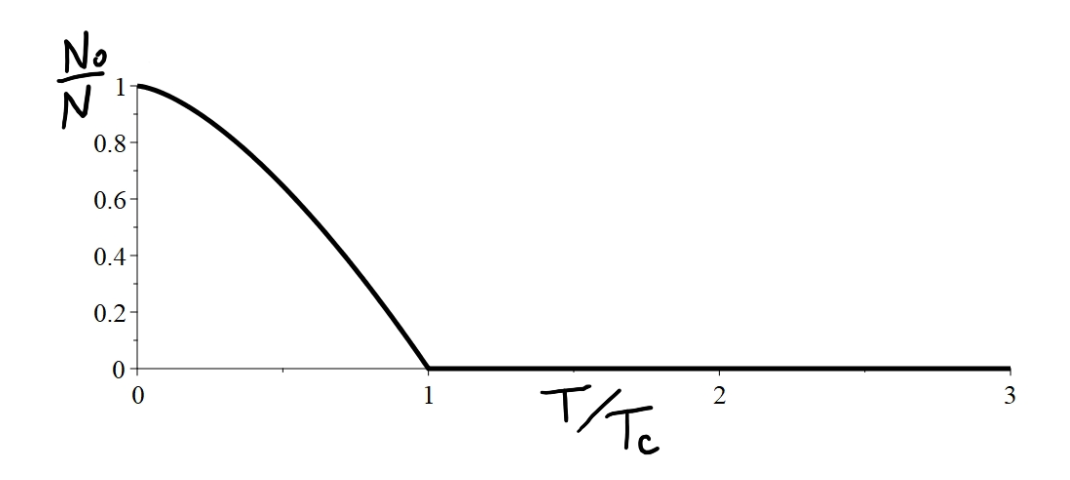
\includegraphics[width=0.7\textwidth]{images/fermi_temp.png}
\end{center}

The ``kink'' in this plot can be regarded as a phase transition.
\gap
\sheader{Above the Phase Transition} First, define \textit{fugacity}:
\begin{align*}
  z = e^{\beta \mu}
\end{align*}
In order to satisfy constraints, it can be assumed that $0 < z < 1$. Reframing something as a series expansion and some other trickery, we retrieve that:
\begin{align*}
  \bar{N} = \frac{V}{h^3}(2\pi mkT)^\frac{3}{2}Li_\frac{3}{2}(z)
\end{align*}
From this, we can extract a relationship for $\mu$:
\begin{align*}
  \frac{N}{V}\frac{h^3}{(2\pi mkT)^\frac{3}{2}} = Li_\frac{3}{2}(e^{\frac{\mu}{kT}})
\end{align*}
Note that $z \approx 0$ is the classical limit.
\gap
We can also identify the average energy:
\begin{align*}
  \bar{E} = \frac{V}{h^3}\frac{3}{2}(2\pi m)^\frac{3}{2} (kT)^\frac{5}{2} Li_\frac{5}{2}(z)
\end{align*}
\vfill\pagebreak
\header{Quantum Field Theory}
For a Quantum Field Theory where there are single particle states $i$ with energy $E_i$, the partition function for this theory is:
\begin{align*}
  Z = \sum_{\curly{n_i}}e^{-\beta(n_i E_i)}
\end{align*}
This is the same as the grand partition function, where $\mu = 0$. It is important to note that we are summing over $\curly{n_i}$, as particle counts aren't fixed. Hence, we can also get the occupation number:
\begin{align*}
  \bar{n}_i = \frac{1}{e^{\beta E_i} - 1}
\end{align*}
It's kind of elusive in the slides, but what we're really trying to get at here are photons. Hence, we can 1d-particle-in-a-box and then run a volume integral, and then all of this converges to a presentation of blackbody radiation:
\begin{align*}
  E\left([f, f + df]\right) &= V \cdot \frac{8\pi h}{c^3} \frac{f^3}{e^{\frac{hf}{kT}} - 1} df\\
  d\rho_E &= \frac{E}{V} = \frac{8\pi h}{c^3}\frac{f^3}{e^\frac{hf}{kT} - 1}df
\end{align*}
To find the energy or flux coming out of a box with flux density $\rho_E$, we can compute:
\begin{align*}
  E &\approx \rho_e \cdot A \cdot c \cdot dt & \text{Flux} \approx \frac{1}{4} c \cdot \rho_E
\end{align*}
The $\frac{1}{4}$ comes from angles, etc.
\gap
And finally, we come back to radiation from an object:
\begin{align*}
  \text{Emitted Energy Flux} &= \varepsilon \frac{1}{4} c \rho_E\\
  &= \varepsilon \sigma T^4
\end{align*}
Where $\varepsilon = 1$ in blackbody radiation, and $\sigma = \frac{2\pi^5k^4}{15h^3c^2}$ (Stefan-Boltzmann Constant).
\gap
\sheader{Radiation Pressure} For a single particle state, we can compute the radiation pressure:
\begin{align*}
  E_{\vec{\kappa}} &= \frac{hc}{2L}|\vec{\kappa}| = \frac{hc}{2V^{1/3}}|\vec{\kappa}|\\
  P_{\vec{\kappa}} &= - \left(\frac{\partial E_{\vec{\kappa}}}{\partial V}\right) = \frac{1}{3}\frac{E_{\vec{\kappa}}}{V}
\end{align*}
And over all $\vec{k}$, this results in:
\begin{align*}
  P = \frac{1}{3}\frac{E}{V} = \frac{8}{3}\pi \frac{k^4}{h^3c^3}T^4
\end{align*}
We can also extract some relationships for how radiation pressure changes with container size, for some cube with side length $a$:
\begin{align*}
  \frac{d\rho_E}{\rho_E} &= -4 \frac{da}{a} & \rho_E = \frac{C}{a^4}
\end{align*}
\vfill\pagebreak
\header{Vibrations in Solids}
Imagine $N$ atoms with interactions. Their Hamiltonian is as follows:
\begin{align*}
  H = \sum_{i} \frac{p_i^2}{2m} + V(x_1, x_2, \ldots, x_{3N})
\end{align*}
If the potential is minimizable, then let $\Delta_i = x_i - x_i^{\text{eq}}$, and thus under a Taylor expansion:
\begin{align*}
  V(x_1, \ldots, x_{3N}) = V_\text{min} + \frac{1}{2}\sum_{i, j} V_{ij}\Delta_i \Delta_j
\end{align*}
We can do this in a matrix form back in the Hamiltonian:
\begin{align*}
  H = \sum_i \frac{p_i^2}{2M} + \frac{1}{2}[\Delta_1 \cdots \Delta_{3N}] \begin{bmatrix}
    V_{11} & V_{12} & \cdots & V_{1, 3N}\\
    V_{21} & &\\
    \vdots & & \\
    V_{3N, 1} & \cdots & \cdots & V_{3N, 3N}
  \end{bmatrix}
  \begin{bmatrix}
    \Delta_1\\
    \vdots\\
    \vdots\\
    \Delta_{3N}
  \end{bmatrix}
\end{align*}
From the $V$ matrix, we can extract its eigenvectors $\hat{v}_a$ and its eigenvalues $\lambda_a$. Such, we can write things in matrix form:
\begin{align*}
  \vec{\Delta} &= \sum_{a} y_a \hat{v}_a & \vec{p} = \sum_a p_a \hat{v}_a && H = \sum_a \frac{p_a^2}{2M} + \frac{1}{2} \sum_a \lambda_a y_a^2.
\end{align*}
These $\vec{\Delta}$ are what we call the ``normal modes'' of the system, and they are all harmonic oscillators with frequency $\ds \omega_a = \sqrt{\frac{\lambda_a}{M}}$. In the quantum case, allowed energies above the ground state are given by $n \cdot \hbar \omega_a$, and we call these \textit{phonons}. They have the exact same occupation number as identical bosons at $\mu = 0$:
\begin{align*}
  n_a = \frac{1}{e^{\beta E_a} - 1}
\end{align*}
Hence, the total energy is given by:
\begin{align*}
  E = \sum_{a} n_a E_a = \sum_{a} \frac{E_a}{e^{\beta E_a} - 1}
\end{align*}
With this, we can show that the energy for a phonon is very similar to that of a single-polarization photon. Let there be 3 polarizations in a phonon, 1 longitudinal, with speed $v_L$, and 2 transverse with speed $v_T$:
\begin{align*}
  E_\text{photon} = V \frac{\pi^2 k^4}{30\hbar^3} T^4 \left(\frac{1}{v_L^3} + \frac{2}{v_T^3}\right)
\end{align*}
We can then arrive at the specific heat for a vibrational solid, in two limits:
\begin{align*}
  C_{T}^\text{Low} &= V \frac{2}{15} \frac{\pi^2 k^4}{\hbar^3} \left(\frac{2}{v_T} + \frac{1}{v_L}\right) \cdot T^3 \propto T^3 & 
  C_T^\text{High} = 3Nk
\end{align*}

\vfill\pagebreak

\header{Spin Interactions}
At a high level overview, there are three overarching physical systems underscoring the physics of solids:
\begin{enumerate}
\item Lattice Vibrations (phonons)
\item Conduction Electrons (bands)
\item Spins/Magnetic Moments (magnetism)
\end{enumerate}
So let's take a look at spins.
\gap
\sheader{Ising Model} Spins can interact! So now we have the Ising model:
\begin{align*}
  H = -h \sum_{i} s_i - J \sum_{\langle i, j \rangle} s_i s_j
\end{align*}
Through this, we wish to find the average magnetization: $\langle s_i \rangle = m(h, J, T)$.
\gap
\sheader{Mean Field Theory} Mean field theory serves as an analytic approximation to solve an ising spin problem. One treats each spin individually and models the rest of the system by some fixed environment. Essentially, this process requires assuming some $m$, calculating $\langle s_i \rangle$ with it, and then requiring that $\langle s_i \rangle = m$. This works in only select cases. To start, we first define the Hamiltonian for a single spin:
\begin{align*}
  H_1 = -(h + Jqm)s \implies Z_1 = \sum_{s = \pm 1}e^{-\beta H_1} = 2 \cosh \left(\beta(h + qJm)\right)
\end{align*}
We can find $\langle s_i \rangle$ with the following expression:
\begin{align*}
  \langle s \rangle = \frac{1}{\beta} \frac{\partial \ln Z}{\partial h} = \tanh \left(\beta (h + qJm)\right)
\end{align*}
And thus, the final step is to solve the following:
\begin{align*}
  m = \tanh \left( \beta (h + qJm)\right)
\end{align*}
This generally has two results:
\begin{enumerate}
\item High $T$: only $m = 0$ is consistent
\item Low $T$: $m = 0$, $m = \pm m_0$
  \begin{itemize}
  \item It is important to note that the $\pm m_0$ states have a lower free energy, so these result in \textit{spontaneous magnetization} and correspond to states of ferromagnets.
  \end{itemize}
\end{enumerate}
We can see this behaviour plotted:
\begin{center}
  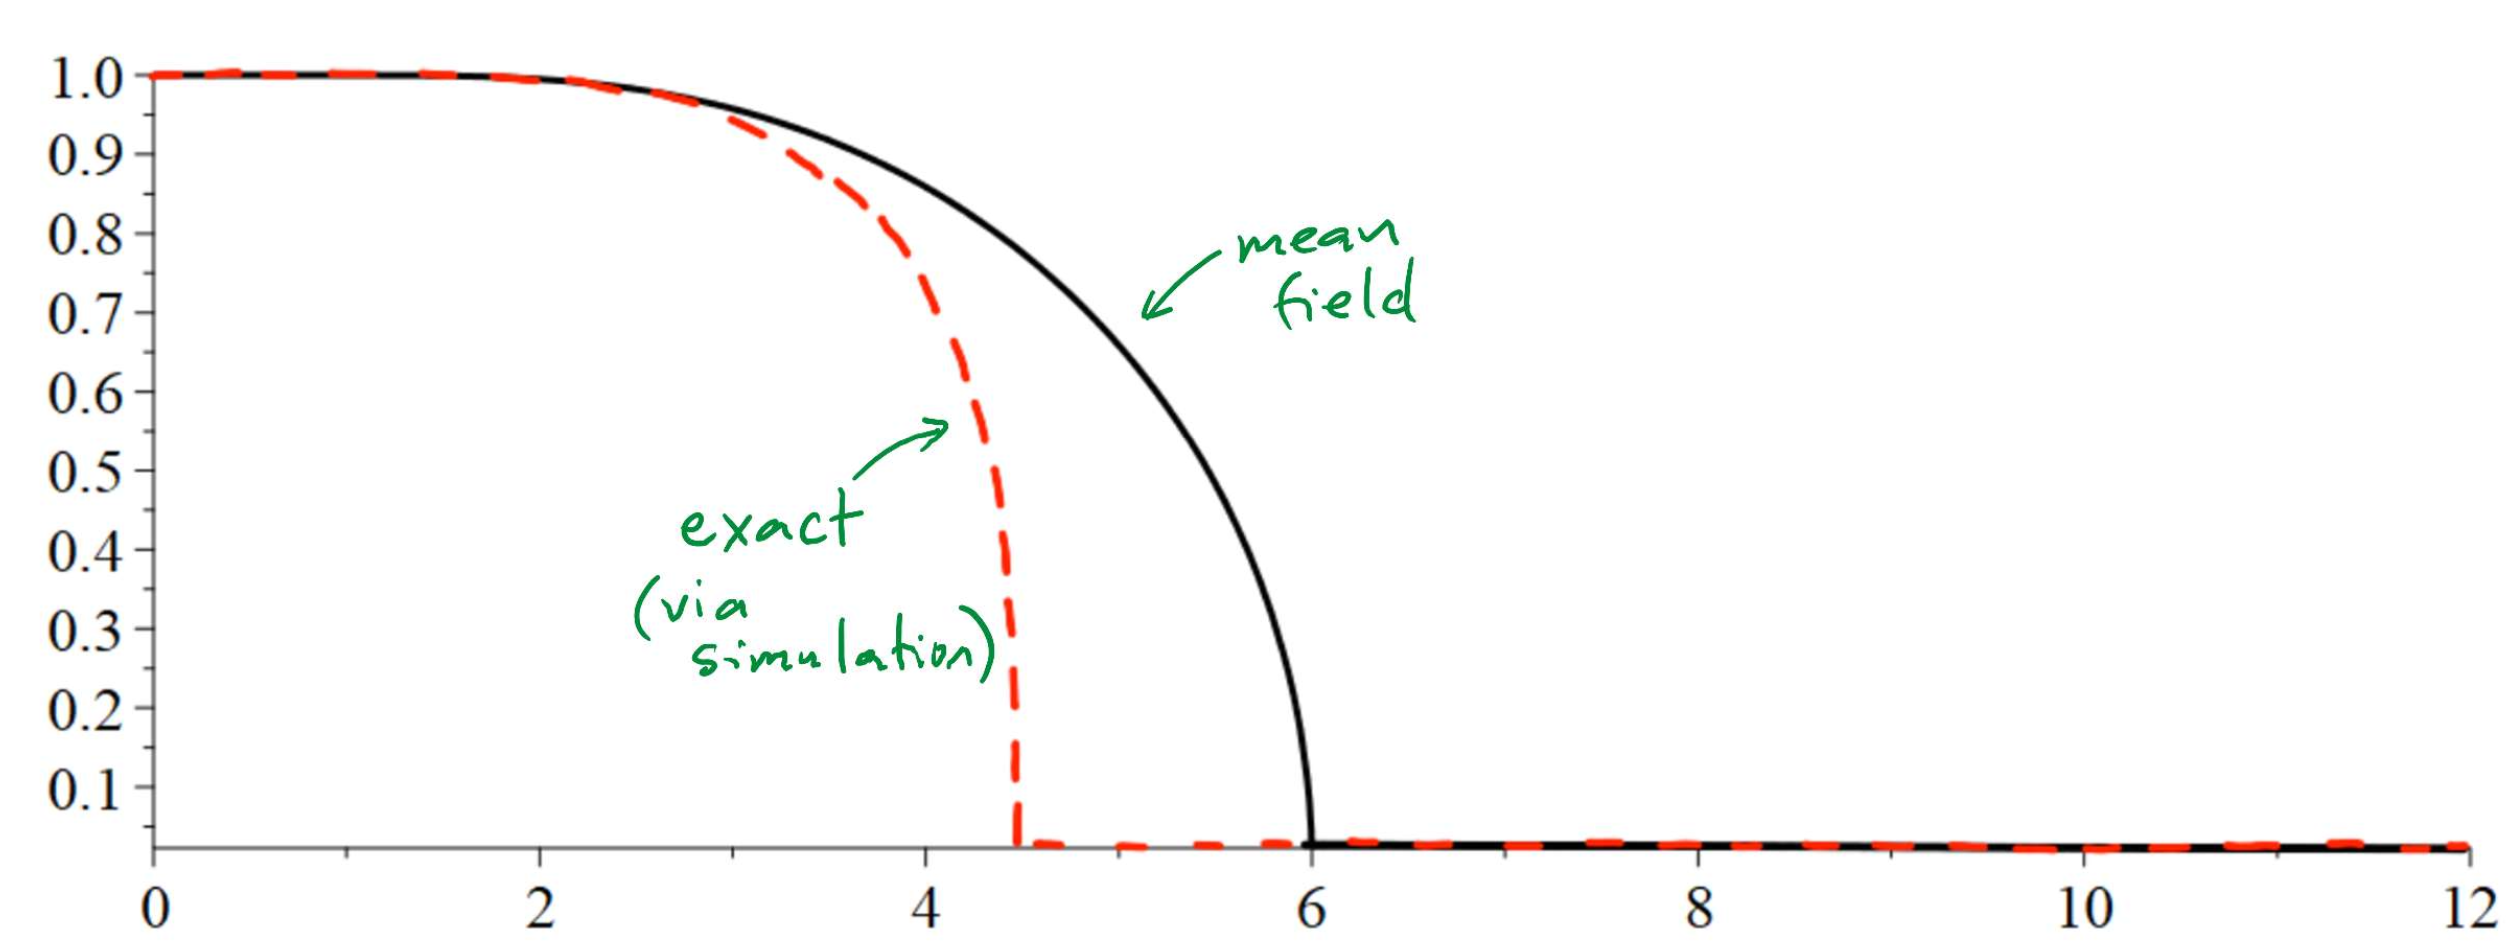
\includegraphics[width=0.7\textwidth]{images/magnet_phase.png}
\end{center}
%% \sheader{Magnetization Problems} Often, you'll get problems that give an array of spins and are asked to provide the magnetization. Count the number of $\pm$ interactions in between the spins.
\sheader{Monte Carlo Simulations} Basically, this trying to calculate the spins explicitly is horrendously computationally expensive. So, we can ``imitate nature'' by doing a Monte Carlo method. Basically, continuously pick random spins, set them to $\pm 1$ with probability calculated from the nearest neighbours, and then repeat, repeat, repeat.
\vfill\pagebreak
\header{Charge Polarization Repulsion}
Basically, polarizations and shifting charge densities in molecules/atoms can have the effect of creating attractive or repulsive forces between molecules. This generally looks like the following:
\begin{center}
  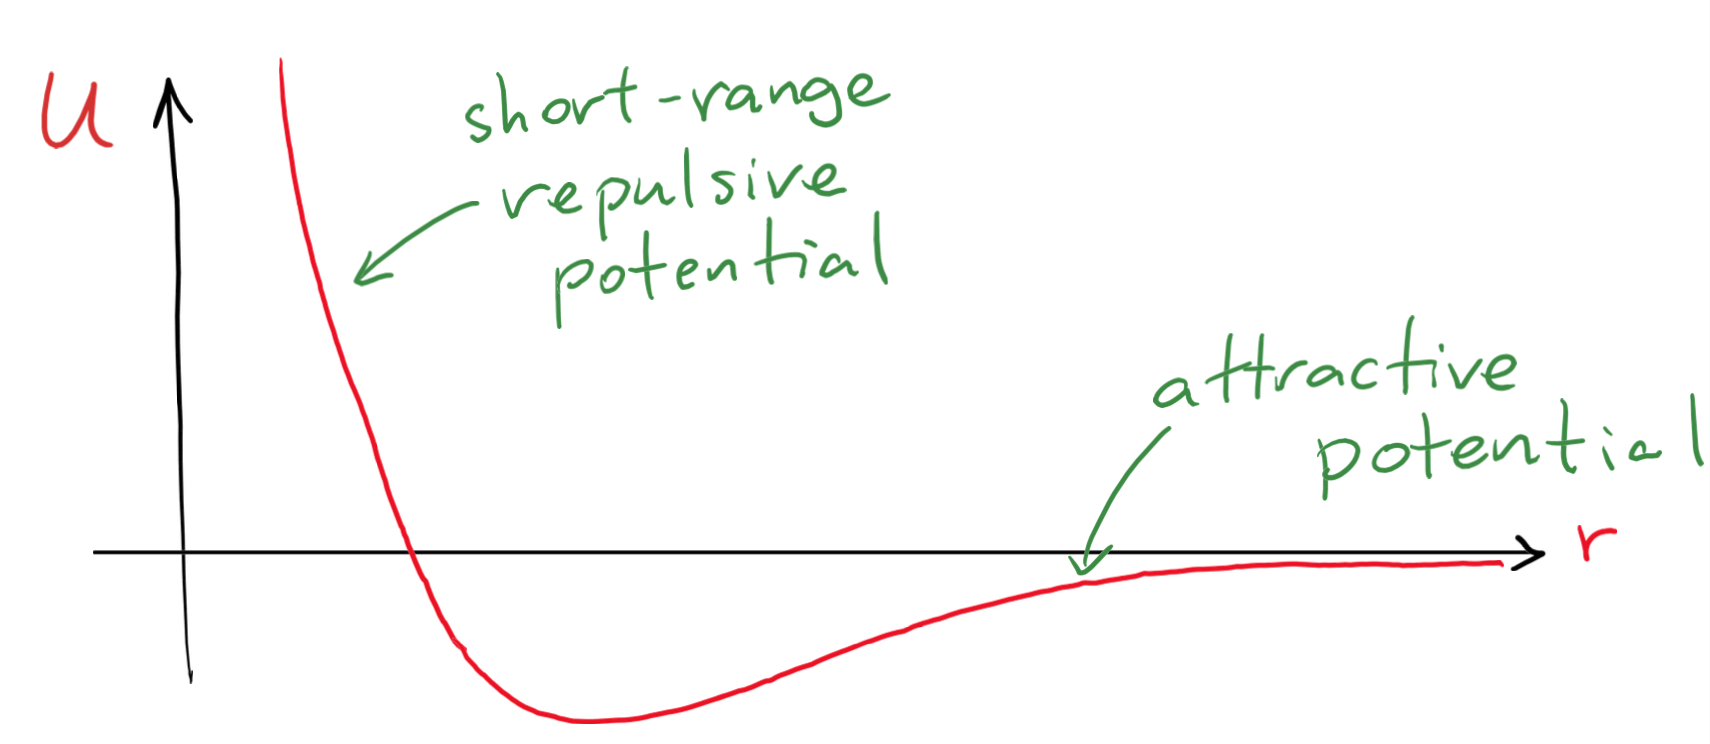
\includegraphics[width=0.6\textwidth]{images/vander.png}
\end{center}
The atrractive potential follows approximatley a $\ds \propto \frac{1}{r^6}$ curve. This comes from electron correlation and dipoles, or London dispersion forces. A bit more handwavey, but some say that the short-range repulsive potential is $\propto \frac{1}{r^12}$. Through a bunch of simplifications, we can find the partition function for a gas with particle interactions:
\begin{align*}
  Z \approx \frac{1}{N!}\frac{1}{h^{3N}} (2\pi m kT)^\frac{3N}{2} \cdot V^N \left(1 - \frac{1}{2} \frac{N^2}{V^2} I_u(T)\right)
\end{align*}
where:
\begin{align*}
  I(T) = \int 4\pi r^2 \left(e^{-\beta U(r)}- 1\right) dr
\end{align*}
If we phrase this in terms of ideal gas law:
\begin{align*}
  P = \frac{NkT}{V} - \frac{1}{2}\frac{N^2}{V^2}I_u(T)
\end{align*}
There's some other funky math here if we investigate the \textit{virial expansion}. Define $n \equiv \frac{N}{V}$, and such, we can take an ``expansion'' of the number density for low densities:
\begin{align*}
  \frac{P}{kT} = n + B_2(T)n^2 + B_3(T)n^3 + \cdots
\end{align*}
This implies that:
\begin{align*}
  B_2(T) = - \frac{1}{2}I_u(T)
\end{align*}
So what is $U$? We can model this for whatever we want to call the potential, but a choice one could make is to look at the long range attractive potential:
\begin{align*}
  U(r) = \begin{cases}
    0 & r < r_0 \\
    -u_0 \frac{r_0^6}{r^6} & r > r_0
  \end{cases}
\end{align*}

\sheader{Mean Field Theory Approach} Turns out, we can apply mean field theory in other places too! First, approximate the partition function for identical particles:
\begin{align*}
  Z = \frac{1}{N!}
\end{align*}
We then approximate the potentials such that there is a small repulse region (orange) and a hard wall (black) around a particle. Everything else is potential zero. The black region has radius $b$ and the orange has radius $a$.
\begin{center}
  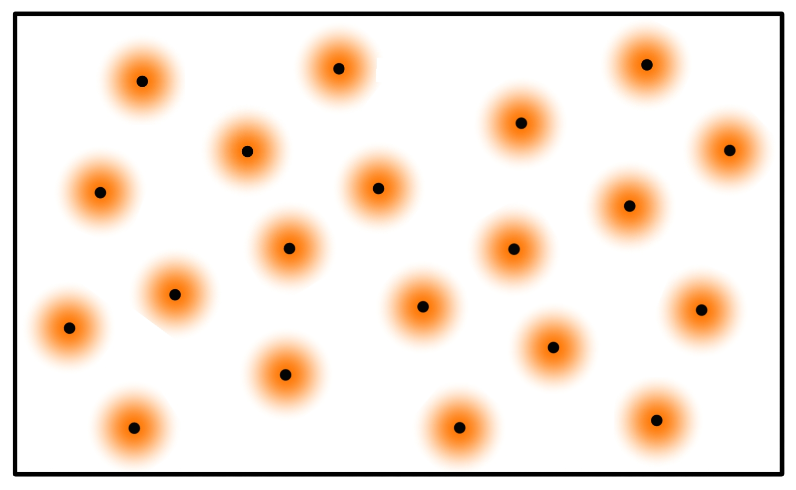
\includegraphics[width=0.5\textwidth]{images/mean_field_gas.png}
\end{center}
Hence, we can then distribute the orange part of the field:
\begin{align*}
  \bar{U} = \frac{-Na}{V-Nb} \approx -\frac{Na}{V}
\end{align*}
\begin{center}
  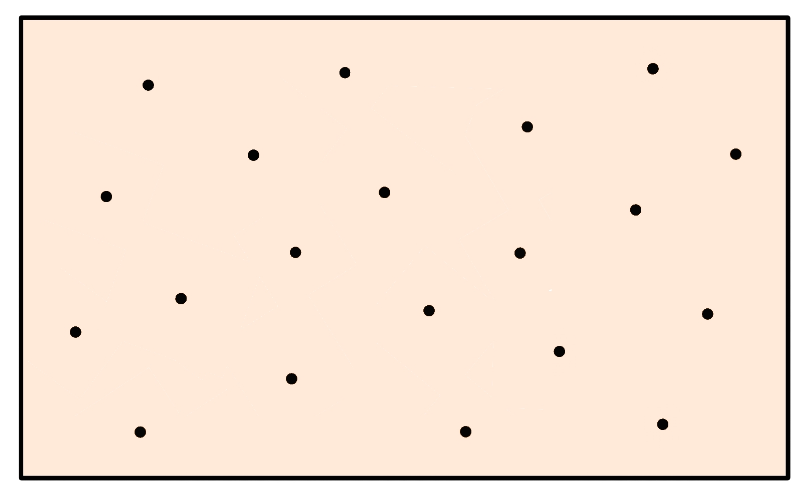
\includegraphics[width=0.5\textwidth]{images/mean_field_smush.png}
\end{center}
Running a spatial integral, we get:
\begin{align*}
  Z_1 = \frac{1}{h^3}\int e^{-\beta \left(\frac{p^2}{2m} + U(\vec{x})\right)} d^3p \cdot d^3x \approx \frac{1}{h^3}(2\pi mkT)^\frac{3}{2}(V - Nb)e^{\beta \frac{N}{V} a}.
\end{align*}
In this case, it follows that:
\begin{align*}
  a &= - \int_{r_0}^{\infty} U(r)(2\pi r^2)dr & b = \frac{2}{3}\pi r^3
\end{align*}
We can find the resultant pressure:
\begin{align*}
  P = - \left(\frac{\partial F}{\partial V}\right)_{T, N} = kt \left(\frac{\partial \ln Z}{\partial V}\right)_{T, N} = \frac{NkT}{V-Nb} - \frac{N^2}{V^2}a
\end{align*}
This is known as the \textit{van der Waals equation of state}. This is equivalent to the expression derived from the initial direct approach with the choice of $U(r)$ described.
\vfill\pagebreak
\header{Phase Transitions}
As we've begun to make modifications to the ideal gas law, an alarming artifact arises: multiple values for volume for a given pressure.
\begin{center}
  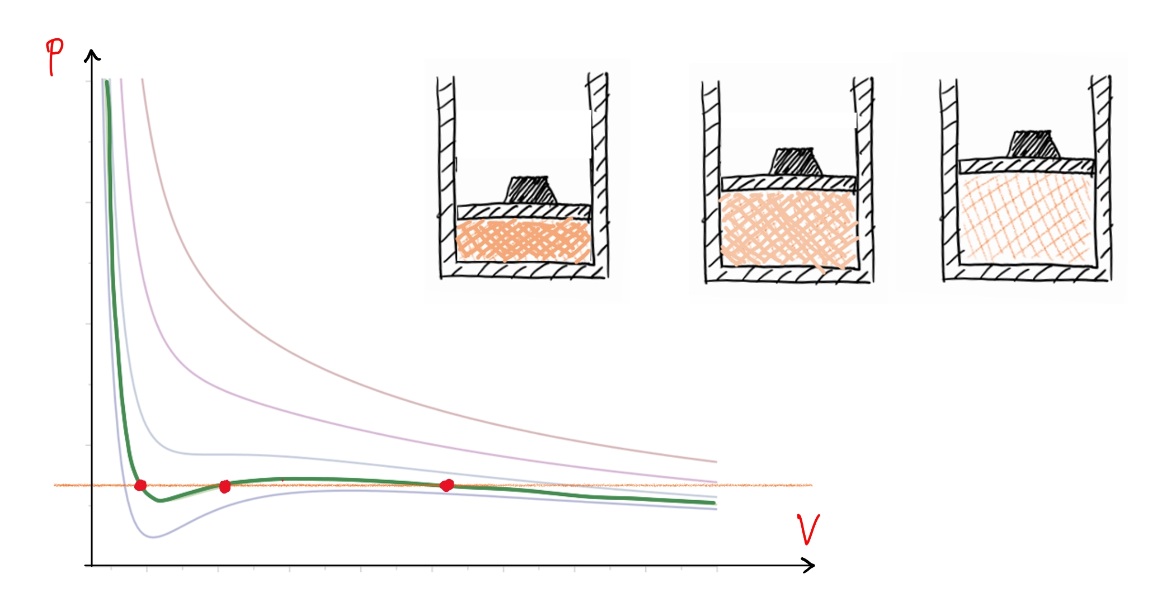
\includegraphics[width=0.6\textwidth]{images/triple_value.png}
\end{center}
This is non-physical, so an explanation is required. It turns out what this ends up representing physically is a coexistence of phases. It is important to note the ``critical point'' on phase diagrams, where three different phases can coexist, and things can become unstable, with large fluctuations in density $\left(\text{Var} \left(\frac{N}{V}\right)\text{ large}\right)$ . This is called \textit{critical opalescence}.
\gap
\sheader{Critical Exponents and Universality} There are some properties that are universal among gases. The first is:
\begin{align*}
  \left(\frac{V}{N}\right)_\text{gas} - \left(\frac{V}{N}\right)_\text{liquid} \sim (T_C - T)^{0.326}
\end{align*}
Another is for the isothermal compressibility:
\begin{align*}
  \kappa_T \sim (T - T_C)^{-1.24} \quad \text{(from above)}
\end{align*}
Anyways, crazy enough, this also works for magnets:
\begin{align*}
  |m| &\sim (T_C - T)^{0.326}\\
  \left(\frac{\partial m}{\partial B}\right)_T &\sim (T - T_c)^{-1.24}
\end{align*}

\header{Einstein's Equations and the Universe}

The universe been \textit{expanding}. We can denote the scale factor $a$ of the universe as how much it's been ``stretching'' since the big bang:
\begin{align*}
  \left[\frac{1}{a} \frac{d}{dt}a\right]^2 = \frac{8\pi G}{c^2}\rho_E
\end{align*}
And also, in the early universe when everything was relativistic:
\begin{align*}
  \rho_E = \frac{C}{a^4}
\end{align*}
The scale factor grew in the early universe as to:
\begin{align*}
  a \propto t^\frac{1}{2}.
\end{align*}

\end{document}
